\documentclass[conference,a4paper]{IEEEtran}

% ---------- Pacotes ----------------------------------------
\usepackage[T1]{fontenc}
\usepackage[utf8]{inputenc}
\usepackage{babel}
\babelprovide[import, main]{portuguese}
\usepackage{graphicx}
\usepackage{booktabs}
\usepackage{tabularx}
\usepackage{amsmath,amssymb}
\usepackage{enumitem}
\usepackage{microtype}
\usepackage[hidelinks]{hyperref}
\usepackage{cite}
\usepackage{stfloats}
\usepackage{float}

% Permite que floats de duas colunas ocupem até 90% do topo da página
\renewcommand{\dbltopfraction}{0.9}
\renewcommand{\dblfloatpagefraction}{0.9}

% ---------- Caminho das figuras ----------------------------
\graphicspath{{figures/}}

% ---------- Metadados --------------------------------------
\title{Sistema de Recuperação Rápida de Informações\\
       em Protocolos de Saúde do SUS\\
       {\large Relatório de Detalhamento --- Rumo ao TRL~1}}

\author{
  \IEEEauthorblockN{Antônio Moreira Pinto, Celso Sacramento,
    João Pedro Porto Campos,\\Laura Gonzaga,
    Leonardo Sá Silveira Lima, Thiago Rocha}
  \IEEEauthorblockA{INF2921 / CIS2114 --- PUC-Rio\\
    Maio de 2026}
}

% ===========================================================
\begin{document}

\maketitle

\begin{abstract}
  Profissionais de saúde do SUS perdem tempo precioso buscando
  informações em protocolos clínicos distribuídos em PDFs
  fragmentados e sem indexação adequada. Este relatório detalha
  a proposta do Grupo~E: um assistente conversacional baseado em
  \textit{Retrieval-Augmented Generation} (RAG) que permite consultar
  protocolos em linguagem natural com respostas fundamentadas nas
  fontes oficiais. São apresentados dois casos de uso, além dos
  requisitos funcionais e não funcionais iniciais do sistema.
\end{abstract}

\IEEEpeerreviewmaketitle

% ---------- Seções -----------------------------------------

\section{Introdução}
\label{sec:intro}

O Sistema Único de Saúde (SUS) é operado por uma ampla rede de
profissionais que dependem de protocolos clínicos padronizados
para a tomada de decisão. Esses protocolos são distribuídos
majoritariamente em formato PDF, resultando em uma base documental
fragmentada e de difícil consulta durante o atendimento. A
dificuldade de acesso rápido a essas informações impacta diretamente
a qualidade e a velocidade do cuidado prestado ao paciente.

Este relatório apresenta o detalhamento inicial de um assistente
conversacional baseado em \textit{Retrieval-Augmented Generation}
(RAG) voltado a profissionais do SUS. As seções seguintes discutem
as soluções existentes (Seção~\ref{sec:related}), a arquitetura
proposta (Seção~\ref{sec:methods}), os requisitos iniciais
(Seção~\ref{sec:req}) e os casos de uso ilustrativos
(Seção~\ref{sec:results}).

% ------------------------------------------------------------------

\section{Contexto e Soluções Existentes}
\label{sec:related}

Os Guias de Referência Rápida elaborados pelo Ministério da Saúde
e pelas Secretarias Municipais compilam critérios diagnósticos,
fluxos de atendimento e condutas terapêuticas~\cite{brasil2023protocolos}.
Entretanto, cada guia pode conter dezenas de páginas disponíveis
apenas em cópias físicas ou PDFs não indexados. Complementarmente,
o \textit{Data Zoom Saúde} disponibiliza microdados estruturados
do DATASUS que podem enriquecer respostas sobre indicadores e
disponibilidade de recursos~\cite{datazoom2024}.

As soluções existentes apresentam limitações relevantes. O
\textit{UpToDate} possui custo de licenciamento elevado e cobertura
limitada de protocolos do contexto brasileiro. O Telessaúde
não oferece interface conversacional e depende de consulta humana
assíncrona. Já os LLMs de uso geral não garantem
rastreabilidade até as fontes oficiais, gerando risco de respostas
desatualizadas ou incorretas~\cite{gao2023survey}.

A oportunidade identificada é combinar acesso conversacional com
fundamentação em documentos oficiais do SUS e integração com dados
estruturados, lacuna que o sistema proposto pretende preencher.

% ------------------------------------------------------------------

\section{Sistema Proposto}
\label{sec:methods}

\subsection{Visão Geral}

A solução é composta por três componentes integrados. O primeiro
realiza a extração e indexação dos Guias de Referência Rápida em
uma base vetorial, enriquecendo cada fragmento com metadados de
origem. O segundo conecta o sistema ao \textit{Data Zoom Saúde}
para recuperação de indicadores epidemiológicos estruturados. O
terceiro é a interface conversacional propriamente dita, que recebe
perguntas em linguagem natural, recupera os fragmentos mais
relevantes e gera respostas contextualizadas por meio de um LLM,
citando as fontes consultadas. A Figura~\ref{fig:mockup} ilustra
uma interação típica com o sistema na interface idealizada.

\begin{figure}[H]
  \centering
  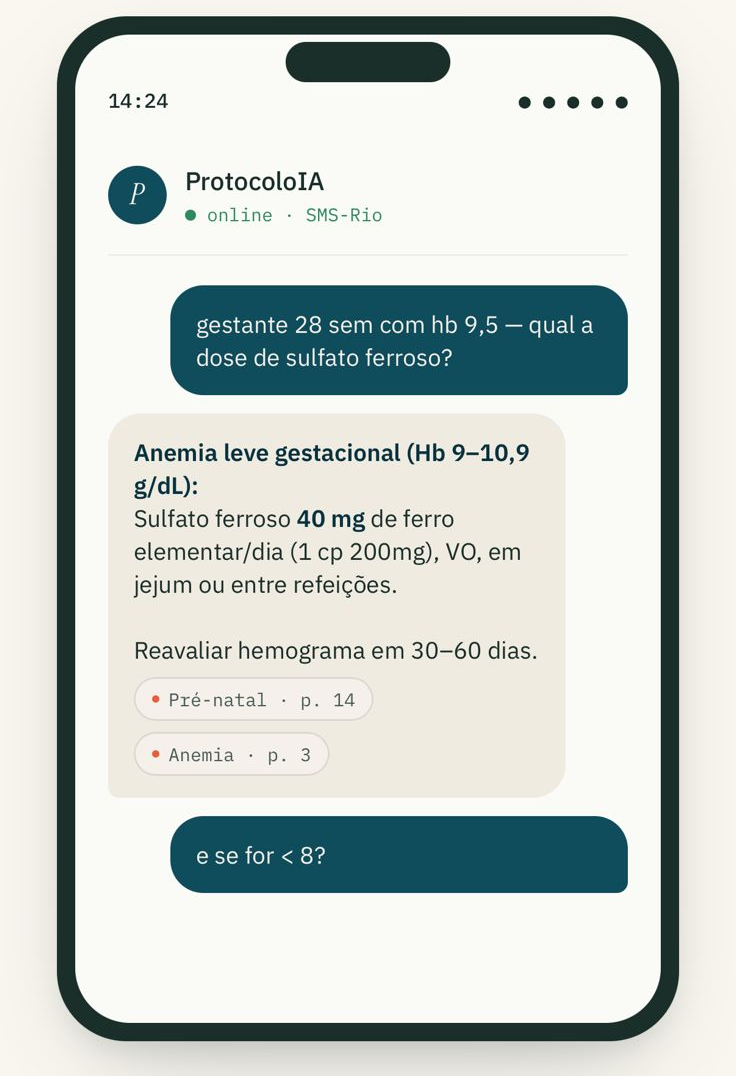
\includegraphics[width=0.6\columnwidth]{../figures/image.png}
  \caption{Mockup da interface conversacional do ProtocoloIA.}
  \label{fig:mockup}
\end{figure}

\subsection{Fontes de Dados}

O sistema opera sobre duas fontes complementares. Os Guias
de Referência Rápida (dado não estruturado) são documentos PDF
produzidos pelo Ministério da Saúde e Secretarias Municipais,
contendo fluxos clínicos e condutas terapêuticas. O \textit{Data
Zoom Saúde} (dado estruturado) oferece microdados do DATASUS
(SIH, SIA, SINAN) sobre produção ambulatorial, internações e
epidemiologia por município.

\subsection{Arquitetura de Recuperação}

O fluxo de consulta segue o padrão RAG~\cite{lewis2020rag}: a
pergunta do usuário é codificada em um vetor $\mathbf{q}$ e cada
fragmento indexado em um vetor $\mathbf{d}$, ambos produzidos por
um modelo de recuperação densa~\cite{karpukhin2020dpr}. Os $k$
fragmentos de maior similaridade do cosseno,

\begin{equation}
  \text{sim}(\mathbf{q}, \mathbf{d}) =
    \frac{\mathbf{q} \cdot \mathbf{d}}{\|\mathbf{q}\|\,\|\mathbf{d}\|},
  \label{eq:cosine}
\end{equation}

são concatenados ao prompt enviado ao LLM, que formula a resposta
final com referências explícitas às fontes consultadas.

\begin{table*}[!t]
  \centering
  \caption{Requisitos funcionais do sistema.}
  \label{tab:req-func}
  \begin{tabularx}{\textwidth}{llX}
    \toprule
    \textbf{ID} & \textbf{Prior.} & \textbf{Descrição} \\
    \midrule
    RF01 & Alta  & Aceitar perguntas em português em linguagem natural, sem exigir conhecimento de sintaxe de busca. \\
    RF02 & Alta  & Recuperar trechos relevantes de PDFs indexados por meio de busca semântica baseada em similaridade vetorial. \\
    RF03 & Alta  & Gerar respostas fundamentadas nos documentos recuperados, citando o documento, seção e página de origem. \\
    RF04 & Alta  & Suportar múltiplos documentos PDF simultaneamente na base vetorial, com atualização incremental. \\
    RF05 & Alta  & Manter contexto de conversação em sessões curtas, permitindo perguntas de acompanhamento sem repetição. \\
    RF06 & Média & Integrar indicadores estruturados do \textit{Data Zoom Saúde} para enriquecer respostas com dados epidemiológicos. \\
    RF07 & Média & Exibir o trecho original do documento ao qual a resposta se refere, possibilitando verificação pela fonte. \\
    RF08 & Média & Indicar nível de confiabilidade da resposta com base na relevância dos fragmentos recuperados. \\
    RF09 & Baixa & Permitir filtragem de consultas por categoria de protocolo (ex.: imunização, saúde mental, hipertensão). \\
    RF10 & Baixa & Oferecer suporte a consultas por voz, convertendo fala em texto antes do processamento. \\
    \bottomrule
  \end{tabularx}
\end{table*}

\begin{table*}[!t]
  \centering
  \caption{Requisitos não funcionais do sistema.}
  \label{tab:req-nfunc}
  \begin{tabularx}{\textwidth}{llX}
    \toprule
    \textbf{ID} & \textbf{Categoria} & \textbf{Descrição} \\
    \midrule
    RNF01 & Usabilidade      & Interface acessível via browser sem instalação adicional, adequada a profissionais sem formação técnica. \\
    RNF02 & Rastreabilidade  & Toda resposta deve citar o documento fonte, seção e página, permitindo verificação e auditoria posterior. \\
    RNF03 & Segurança        & Dados clínicos identificáveis do paciente não devem ser incluídos nas consultas enviadas ao LLM nem nos logs. \\
    RNF04 & Confiabilidade   & O sistema deve indicar explicitamente quando não há informação suficiente nos documentos indexados. \\
    RNF05 & Escalabilidade   & A arquitetura deve suportar a inclusão de novos documentos sem reprocessamento total da base vetorial. \\
    RNF06 & Conformidade     & O sistema deve aderir à LGPD no tratamento de dados de acesso e de identificação de usuários. \\
    RNF07 & Manutenibilidade & Os documentos indexados devem poder ser atualizados independentemente, refletindo novas versões dos protocolos. \\
    \bottomrule
  \end{tabularx}
\end{table*}

% ------------------------------------------------------------------

\section{Requisitos do Sistema}
\label{sec:req}

A Tabela~\ref{tab:req-func} classifica os requisitos
funcionais por prioridade: alta prioridade compõe o núcleo do MVP a
ser validado na primeira iteração; média prioridade agrega valor sem
bloquear essa validação; baixa prioridade fica reservada para versões
subsequentes. A Tabela~\ref{tab:req-nfunc} organiza os requisitos não
funcionais por categoria de qualidade. Rastreabilidade e segurança
recebem atenção especial em razão das implicações clínicas do domínio
e da obrigação de conformidade com a LGPD.

% ------------------------------------------------------------------

\section{Casos de Uso}
\label{sec:results}

\subsection{Caso de Uso 1: Consulta de Protocolo Clínico}

Um médico da Atenção Primária, durante uma consulta, questiona o
sistema sobre o protocolo de tratamento para hipertensão arterial
sistêmica sem comorbidades. O assistente recupera os trechos
pertinentes do Guia de Referência Rápida da SMS e apresenta a
conduta recomendada com indicação da página e versão do documento,
sem que o profissional precise interromper o atendimento para abrir
o PDF manualmente.

\subsection{Caso de Uso 2: Consulta do Calendário de Vacinação}

Uma enfermeira de UBS precisa confirmar o esquema vacinal para
uma criança de 15 meses que chegou sem cartão de vacinação. Ao
descrever a situação ao assistente, recebe uma lista estruturada
das vacinas indicadas pelo Programa Nacional de Imunizações (PNI),
com doses, vias de administração e intervalos mínimos, referenciada
à versão vigente do calendário oficial.

% ------------------------------------------------------------------

\section{Próximas Etapas}
\label{sec:next}

O presente relatório situa o projeto no TRL~1, com a proposta
conceitual formalizada em requisitos e casos de uso. As etapas
previstas são:

\begin{enumerate}[label=\arabic*.]
  \item \textbf{Protótipo de recuperação} (TRL~2): indexação de um
        subconjunto dos Guias de Referência Rápida em uma base vetorial
        local e avaliação qualitativa da relevância dos fragmentos
        recuperados.
  \item \textbf{Validação com usuários} (TRL~3): sessões de uso com
        profissionais de saúde para aferir usabilidade e corretude
        percebida das respostas geradas.
\end{enumerate}

% ---------- Referências ------------------------------------
\bibliographystyle{IEEEtran}
\bibliography{references}

\end{document}
